\documentclass[11pt, xcolor={dvipsnames}, usepdftitle=false]{beamer}
\usepackage{presentation}
\usepackage{graphicx}
\usepackage{array}
\usepackage{booktabs}
\usepackage{hyperref}

\graphicspath{{../Data/}}
\hypersetup{
    pdfpagemode=UseNone,
    hidelinks,
    pdfdisplaydoctitle=true,
    pdftitle={Can Nuclear Fusion Power a Mars Colony?}
}

\title{Can Nuclear Fusion Power a Mars Colony?}
\author{Vineet Reddy, Samuel Heinz, Nicholas Fitzpatrick}
\date{INDENG 290, Spring 2026}
\paperurl{https://github.com/sjheinz17/MarsColonyNuclearFusion}

\begin{document}

\frame{\titlepage}

\begin{frame}
\frametitle{project question}
\begin{itemize}
\item A Mars colony needs steady electric power for life support, oxygen generation, water recycling, lighting, communication, and thermal control.
\item The hard part is that Mars gives us weak sunlight, long nights, and dust storms that can knock down solar output for long stretches.
\item We asked whether fusion belongs in that conversation, or if the realistic answer is still solar plus fission.
\end{itemize}
\end{frame}

\begin{frame}
\frametitle{why this matters}
\begin{itemize}
\item Power is one of the first bottlenecks for any serious colony plan because almost every survival system depends on it.
\item A small outage on Earth is inconvenient, but a long outage on Mars can cut into air, water, and heat.
\item That makes this more than a cost question, it is also a reliability and scaling question.
\end{itemize}
\end{frame}

\begin{frame}
\frametitle{what we compare}
\scriptsize
\begin{tabular}{>{\raggedright\arraybackslash}p{1.65in}>{\raggedright\arraybackslash}p{3.1in}}
\toprule
Option & Why it is in the project \\
\midrule
Solar PV & Already used in space systems, but very exposed to dust and night cycles on Mars. \\
Kilopower class fission & The most realistic near term continuous power option for a Mars surface mission. \\
CFS SPARC & Large tokamak concept that looks strong on projected scale if fusion works. \\
Princeton FRC & Compact fusion concept with a cleaner mass story than a big tokamak. \\
Avalanche Orbitron & Very early compact fusion concept included as a high risk comparison. \\
\bottomrule
\end{tabular}
\end{frame}

\begin{frame}
\frametitle{three project questions}
\begin{enumerate}
\item When does fusion start to look better than just scaling fission.
\item How badly do dust storms hurt reliability.
\item Which fusion concept looks most promising on paper.
\end{enumerate}

\vspace{0.3cm}
\begin{itemize}
\item The final project answers those with feasibility scoring, cost modeling, Monte Carlo reliability simulation, and a smaller forecast comparison.
\end{itemize}
\end{frame}

\begin{frame}
\frametitle{data sources}
\begin{itemize}
\item The downloaded inputs are \texttt{MDAD.csv} from the Mars Dust Activity Database and \texttt{nuclear\_capacity\_data\_annual.csv} from the EIA annual table.
\item The habitat constants, storage assumptions, dust penalty curve, and fusion specs are project tables built from the engineering literature we cite in the report.
\item We kept a plain source record in \texttt{docs/DATA\_SOURCES.md} so the repo shows what was downloaded and what we assembled ourselves.
\end{itemize}
\end{frame}

\begin{frame}
\frametitle{workflow}
\begin{enumerate}
\item Build colony demand assumptions for 6 person, 100 person, and 2{,}000 person cases.
\item Compare power options with a feasibility chart and an all in LCOE model.
\item Run a sol by sol reliability simulation over one Mars year with sampled dust storms.
\item Check scaling and sensitivity results, then summarize the forecast side analysis.
\end{enumerate}
\end{frame}

\begin{frame}
\frametitle{colony demand setup}
\begin{columns}[T]
\begin{column}{0.56\textwidth}
\begin{itemize}
\item Demand includes habitat loads, water recycling, oxygen production, lighting, medical load, communication, and thermal control.
\item We model three colony scales so the project is not locked to a tiny outpost.
\item This gives us a way to ask when the logistics of many small fission units start to look awkward.
\end{itemize}
\end{column}
\begin{column}{0.40\textwidth}
\small
\begin{tabular}{lr}
\toprule
Case & Crew \\
\midrule
Baseline & 6 \\
Mid scale & 100 \\
Large scale & 2{,}000 \\
\bottomrule
\end{tabular}
\end{column}
\end{columns}
\end{frame}

\begin{frame}
\frametitle{reliability model}
\begin{itemize}
\item The reliability model runs one Mars year, 668 sols, and tracks generation, battery state of charge, and unmet demand.
\item Storm sequences come from the Jezero relevant subset of the dust database, then solar is reduced again with a seasonal dust penalty curve.
\item Fission is treated as the stable backbone source, while solar and storage absorb the weather risk.
\end{itemize}
\end{frame}

\begin{frame}
\frametitle{cost and feasibility model}
\begin{itemize}
\item The feasibility chart is a McKelvey style resource view with certainty of existence on one axis and chance of commerciality on the other.
\item The cost model uses an all in levelized cost of energy with capital cost, launch cost, operations, lifetime, and capacity factor.
\item Launch cost matters a lot for Mars, so we include it directly instead of treating it like a side note.
\end{itemize}
\end{frame}

\begin{frame}
\frametitle{forecast side analysis}
\begin{itemize}
\item We also compared three simple forecast approaches on the synthetic colony demand signal.
\item This is not the main result of the project, but it gives one more check that the demand pattern behaves the way we think it does.
\item The models are a constant baseline, a seasonal proxy labeled SARIMA, and a smoothed residual proxy labeled Transformer.
\end{itemize}
\end{frame}

\begin{frame}
\heading{results}
\end{frame}

\begin{frame}
\frametitle{resource view}
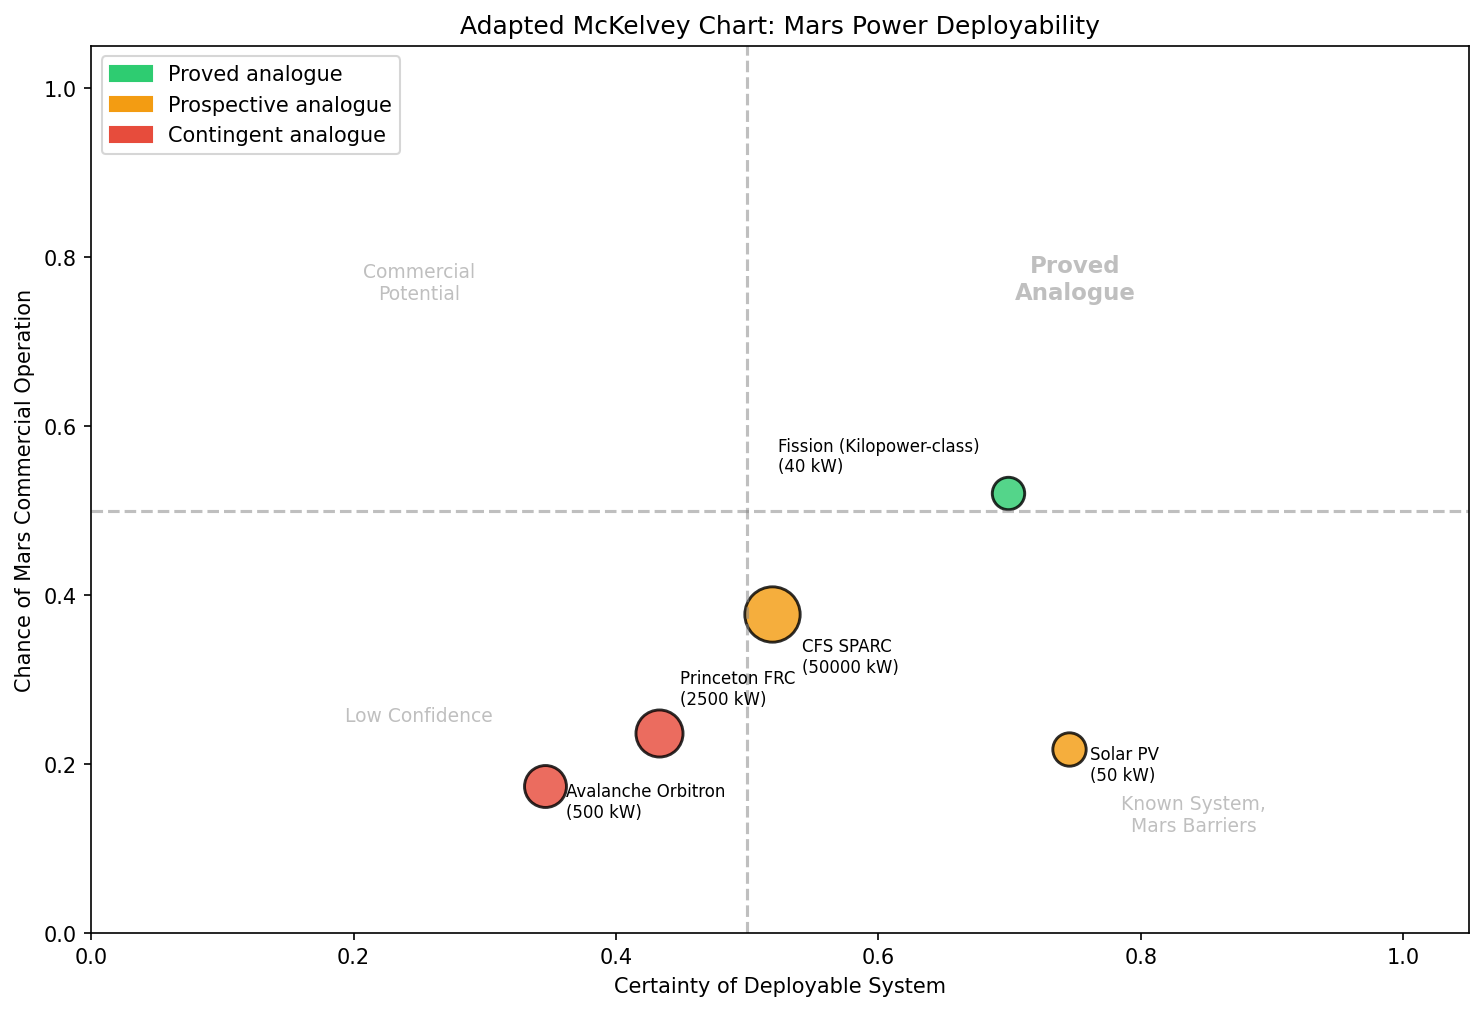
\includegraphics[height=0.56\textheight]{mckelvey_box.png}

\vspace{0.15cm}
\small
\begin{itemize}
\item Fission is the only option that lands in the high certainty and high commerciality corner.
\item Fusion concepts look interesting, but they still sit in the contingent part of the chart because the engineering is not mature yet.
\end{itemize}
\end{frame}

\begin{frame}
\frametitle{cost view}
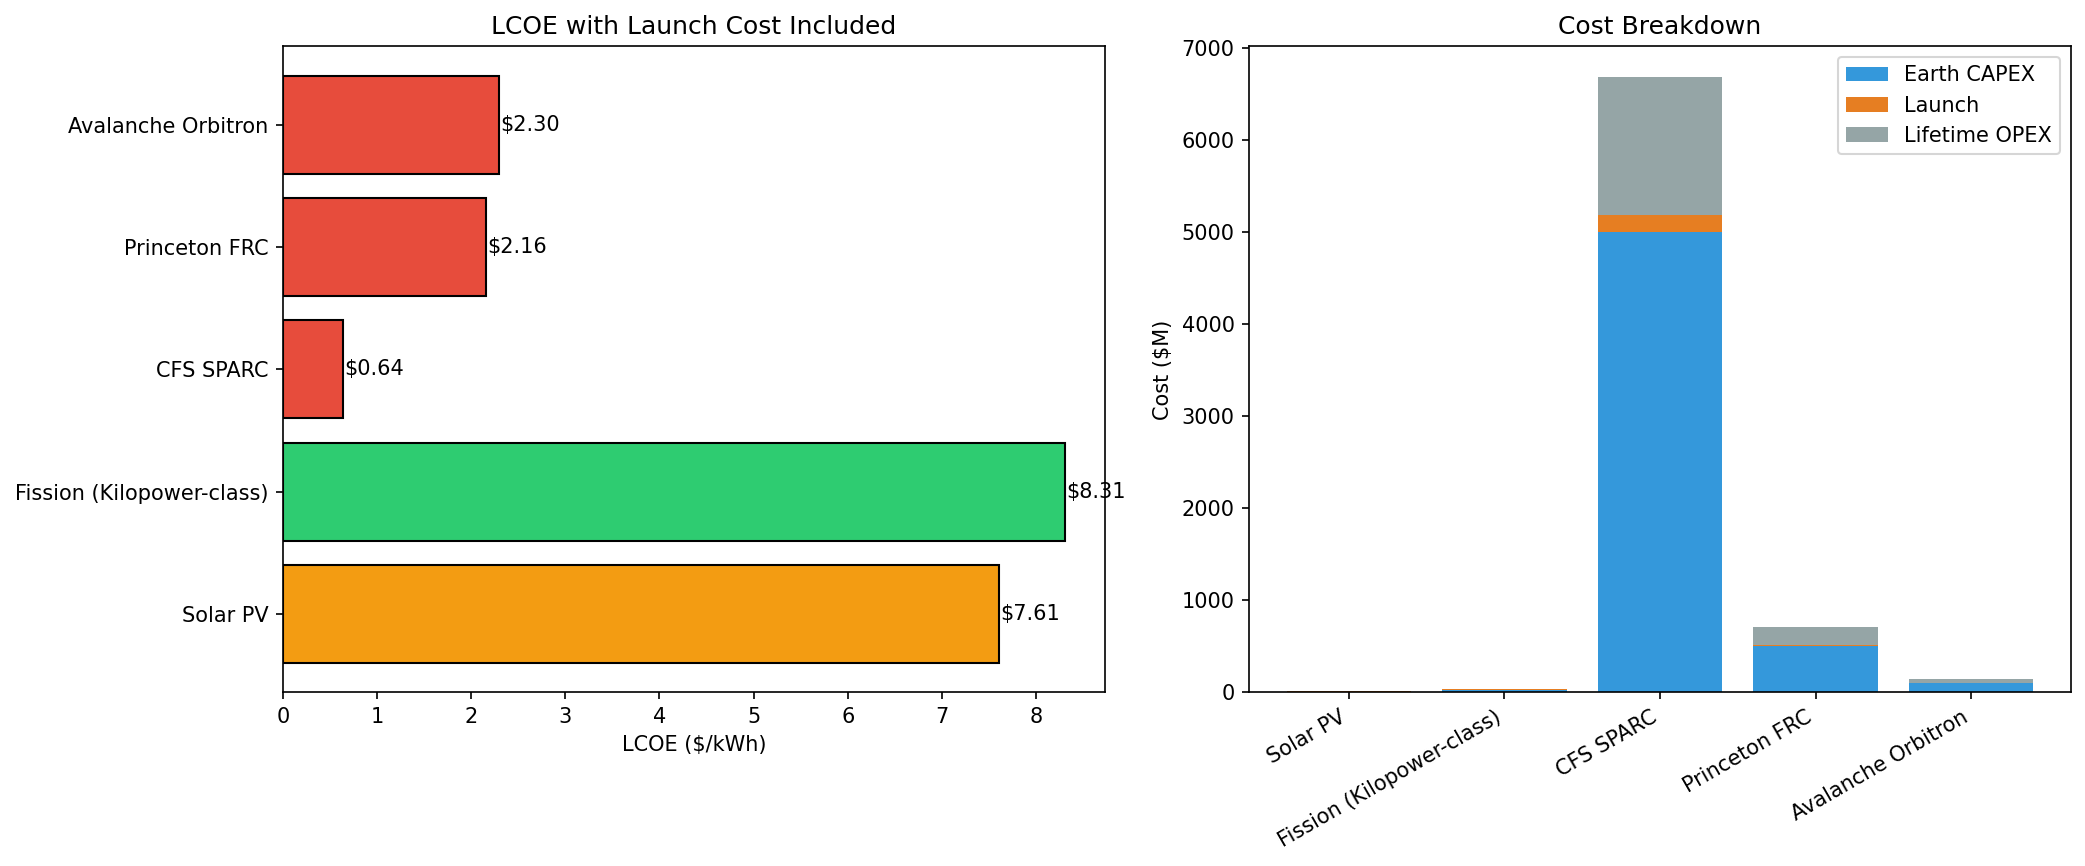
\includegraphics[width=\textwidth]{lcoe_comparison.png}

\vspace{0.15cm}
\begin{itemize}
\item The projected cost picture is almost the reverse of the feasibility picture.
\item SPARC style fusion looks cheapest on paper, but that result depends on a technology we do not have in operation yet.
\end{itemize}
\end{frame}

\begin{frame}
\frametitle{what the cost figure means}
\small
\begin{tabular}{>{\raggedright\arraybackslash}p{2.35in}r}
\toprule
Source & LCOE (\$/kWh) \\
\midrule
Solar PV & 7.61 \\
Kilopower class fission & 8.31 \\
CFS SPARC & 0.64 \\
Princeton FRC & 2.16 \\
Avalanche Orbitron & 2.30 \\
\bottomrule
\end{tabular}

\vspace{0.25cm}
\begin{itemize}
\item The cost model says fusion is attractive only if its published concept numbers are even roughly achievable.
\item That is why the project keeps cost and maturity as two separate lenses.
\end{itemize}
\end{frame}

\begin{frame}
\frametitle{baseline reliability}
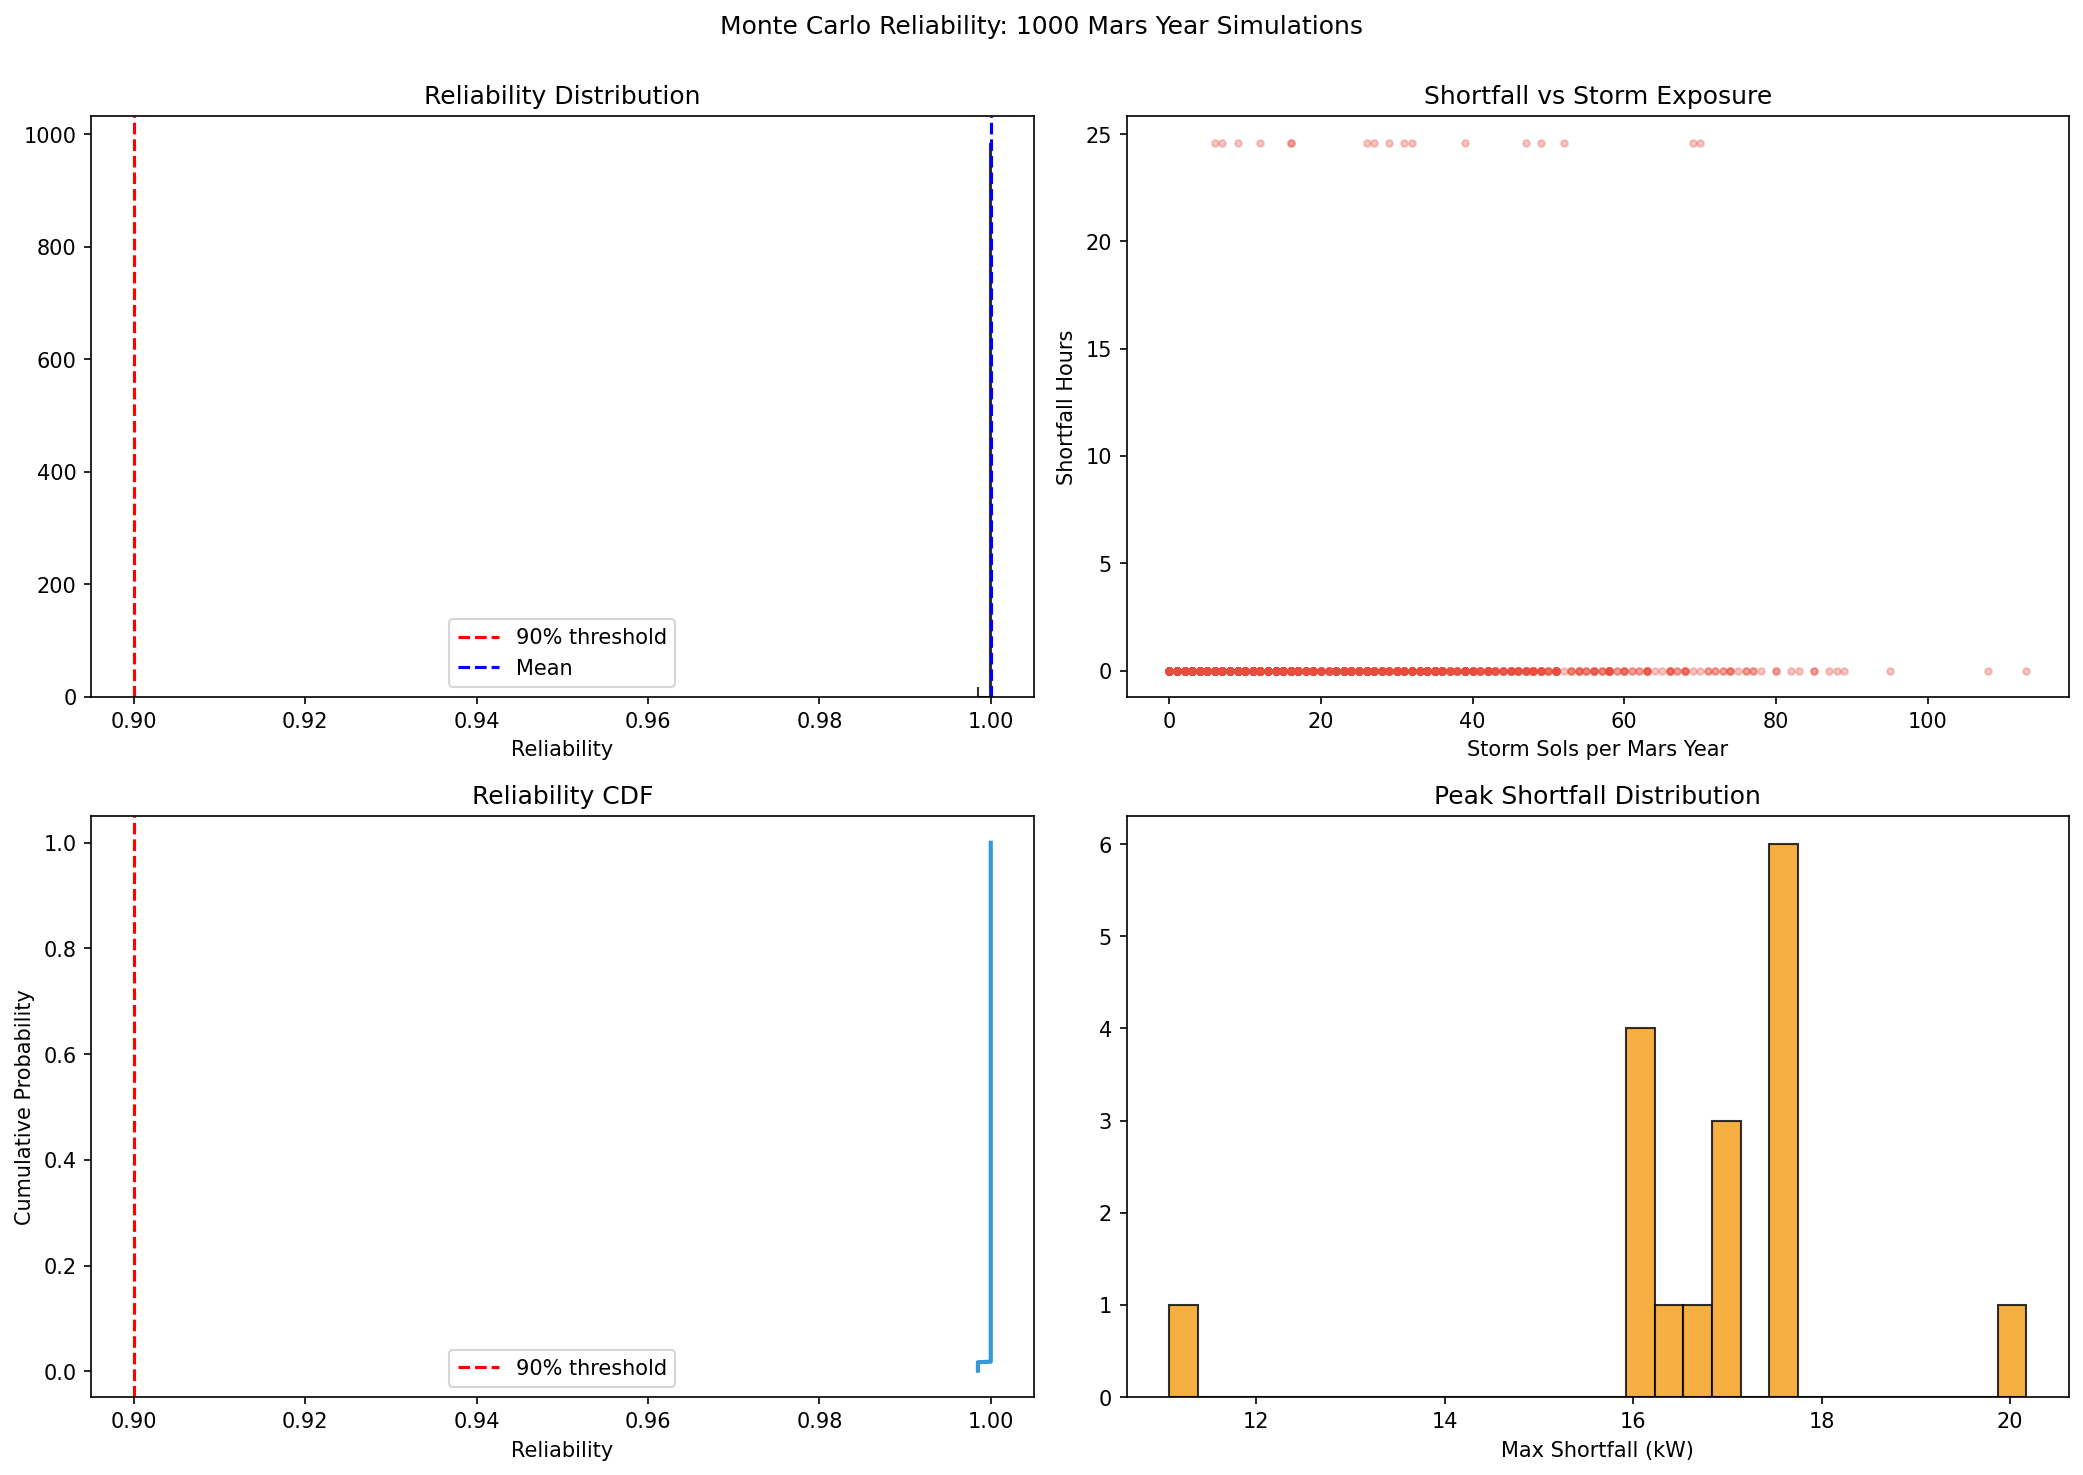
\includegraphics[height=0.56\textheight]{monte_carlo_reliability.png}

\vspace{0.15cm}
\small
\begin{itemize}
\item The 6 person solar plus fission baseline is basically fully reliable across the Monte Carlo runs.
\item This gives us a sanity check before we move to the larger scenario comparison.
\end{itemize}
\end{frame}

\begin{frame}
\frametitle{reliability by scenario}
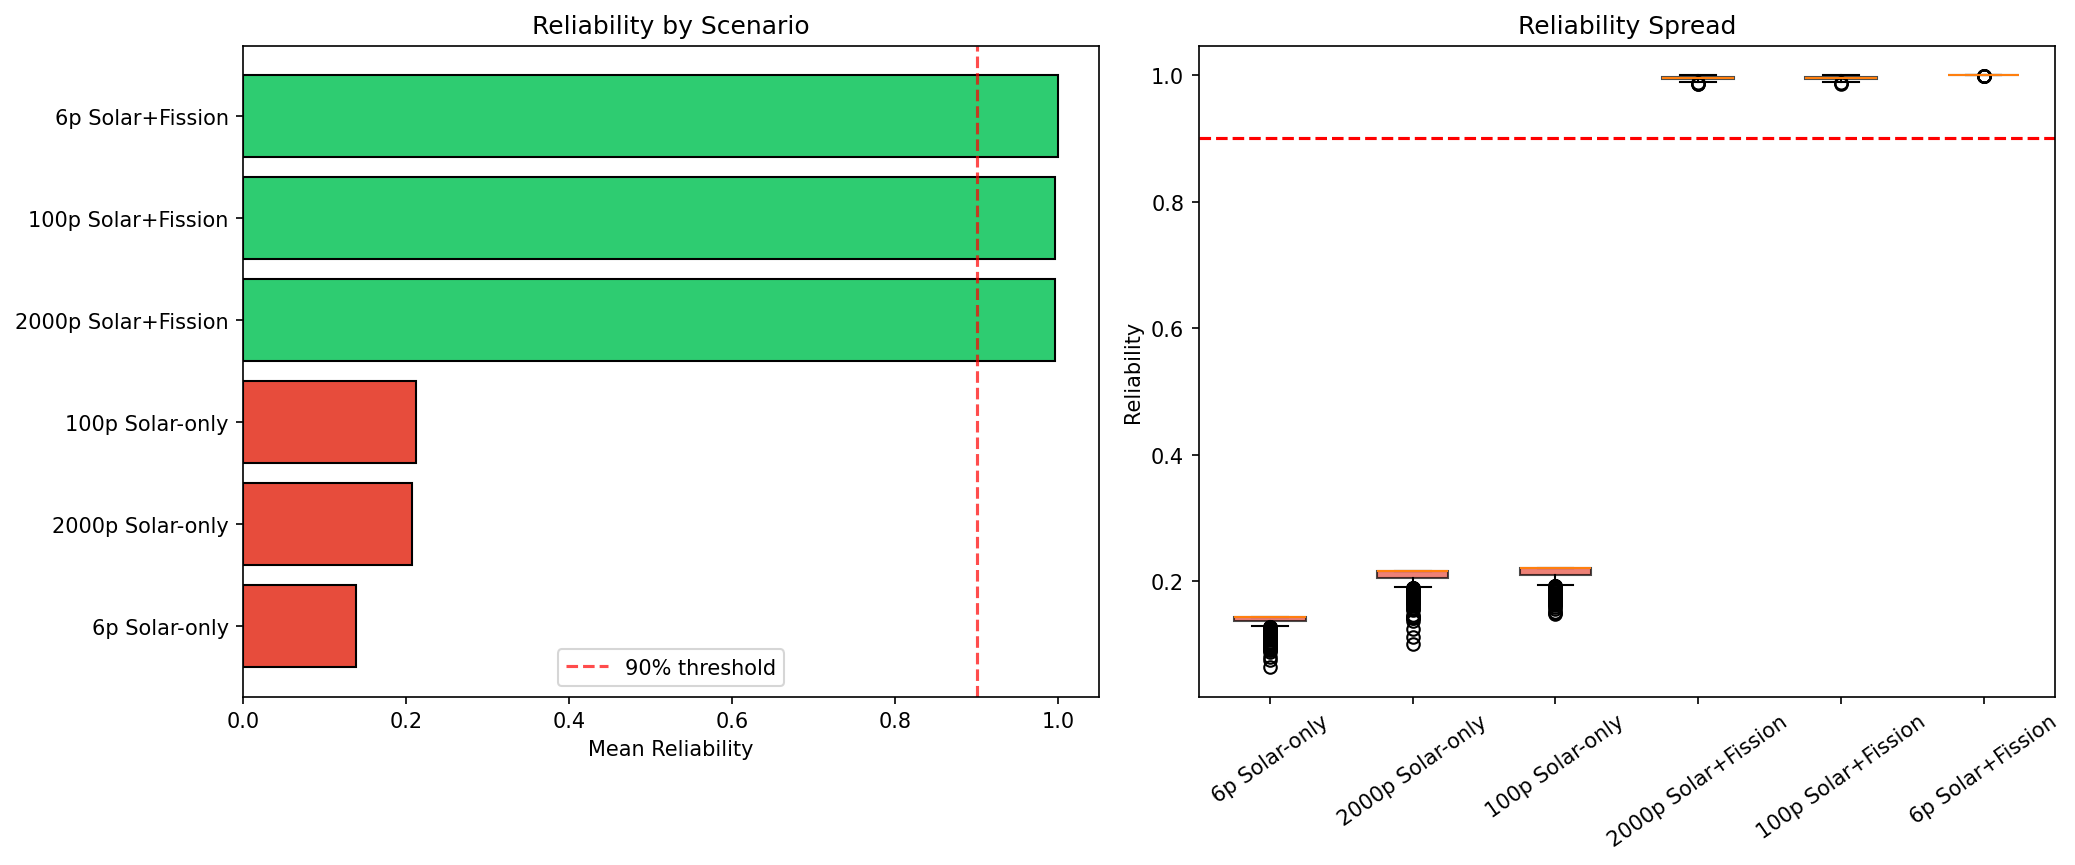
\includegraphics[width=\textwidth]{scenario_reliability.png}

\vspace{0.15cm}
\begin{itemize}
\item The pattern is very stable: solar only cases are weak, and solar plus fission stays near full reliability.
\item That result holds from the 6 person case all the way to the 2{,}000 person case.
\end{itemize}
\end{frame}

\begin{frame}
\frametitle{key reliability numbers}
\small
\begin{tabular*}{\textwidth}{@{\extracolsep\fill}>{\raggedright\arraybackslash}p{2.55in}rr}
\toprule
Scenario & Mean reliability & 5th percentile \\
\midrule
6p Solar only & 0.1379 & 0.1107 \\
6p Solar plus Fission & 1.0000 & 1.0000 \\
100p Solar only & 0.2123 & 0.1796 \\
100p Solar plus Fission & 0.9960 & 0.9910 \\
2000p Solar only & 0.2068 & 0.1751 \\
2000p Solar plus Fission & 0.9958 & 0.9910 \\
\bottomrule
\end{tabular*}

\vspace{0.2cm}
\begin{itemize}
\item The exact values move a little by colony size, but the ranking does not change.
\end{itemize}
\end{frame}

\begin{frame}
\frametitle{scaling pressure}
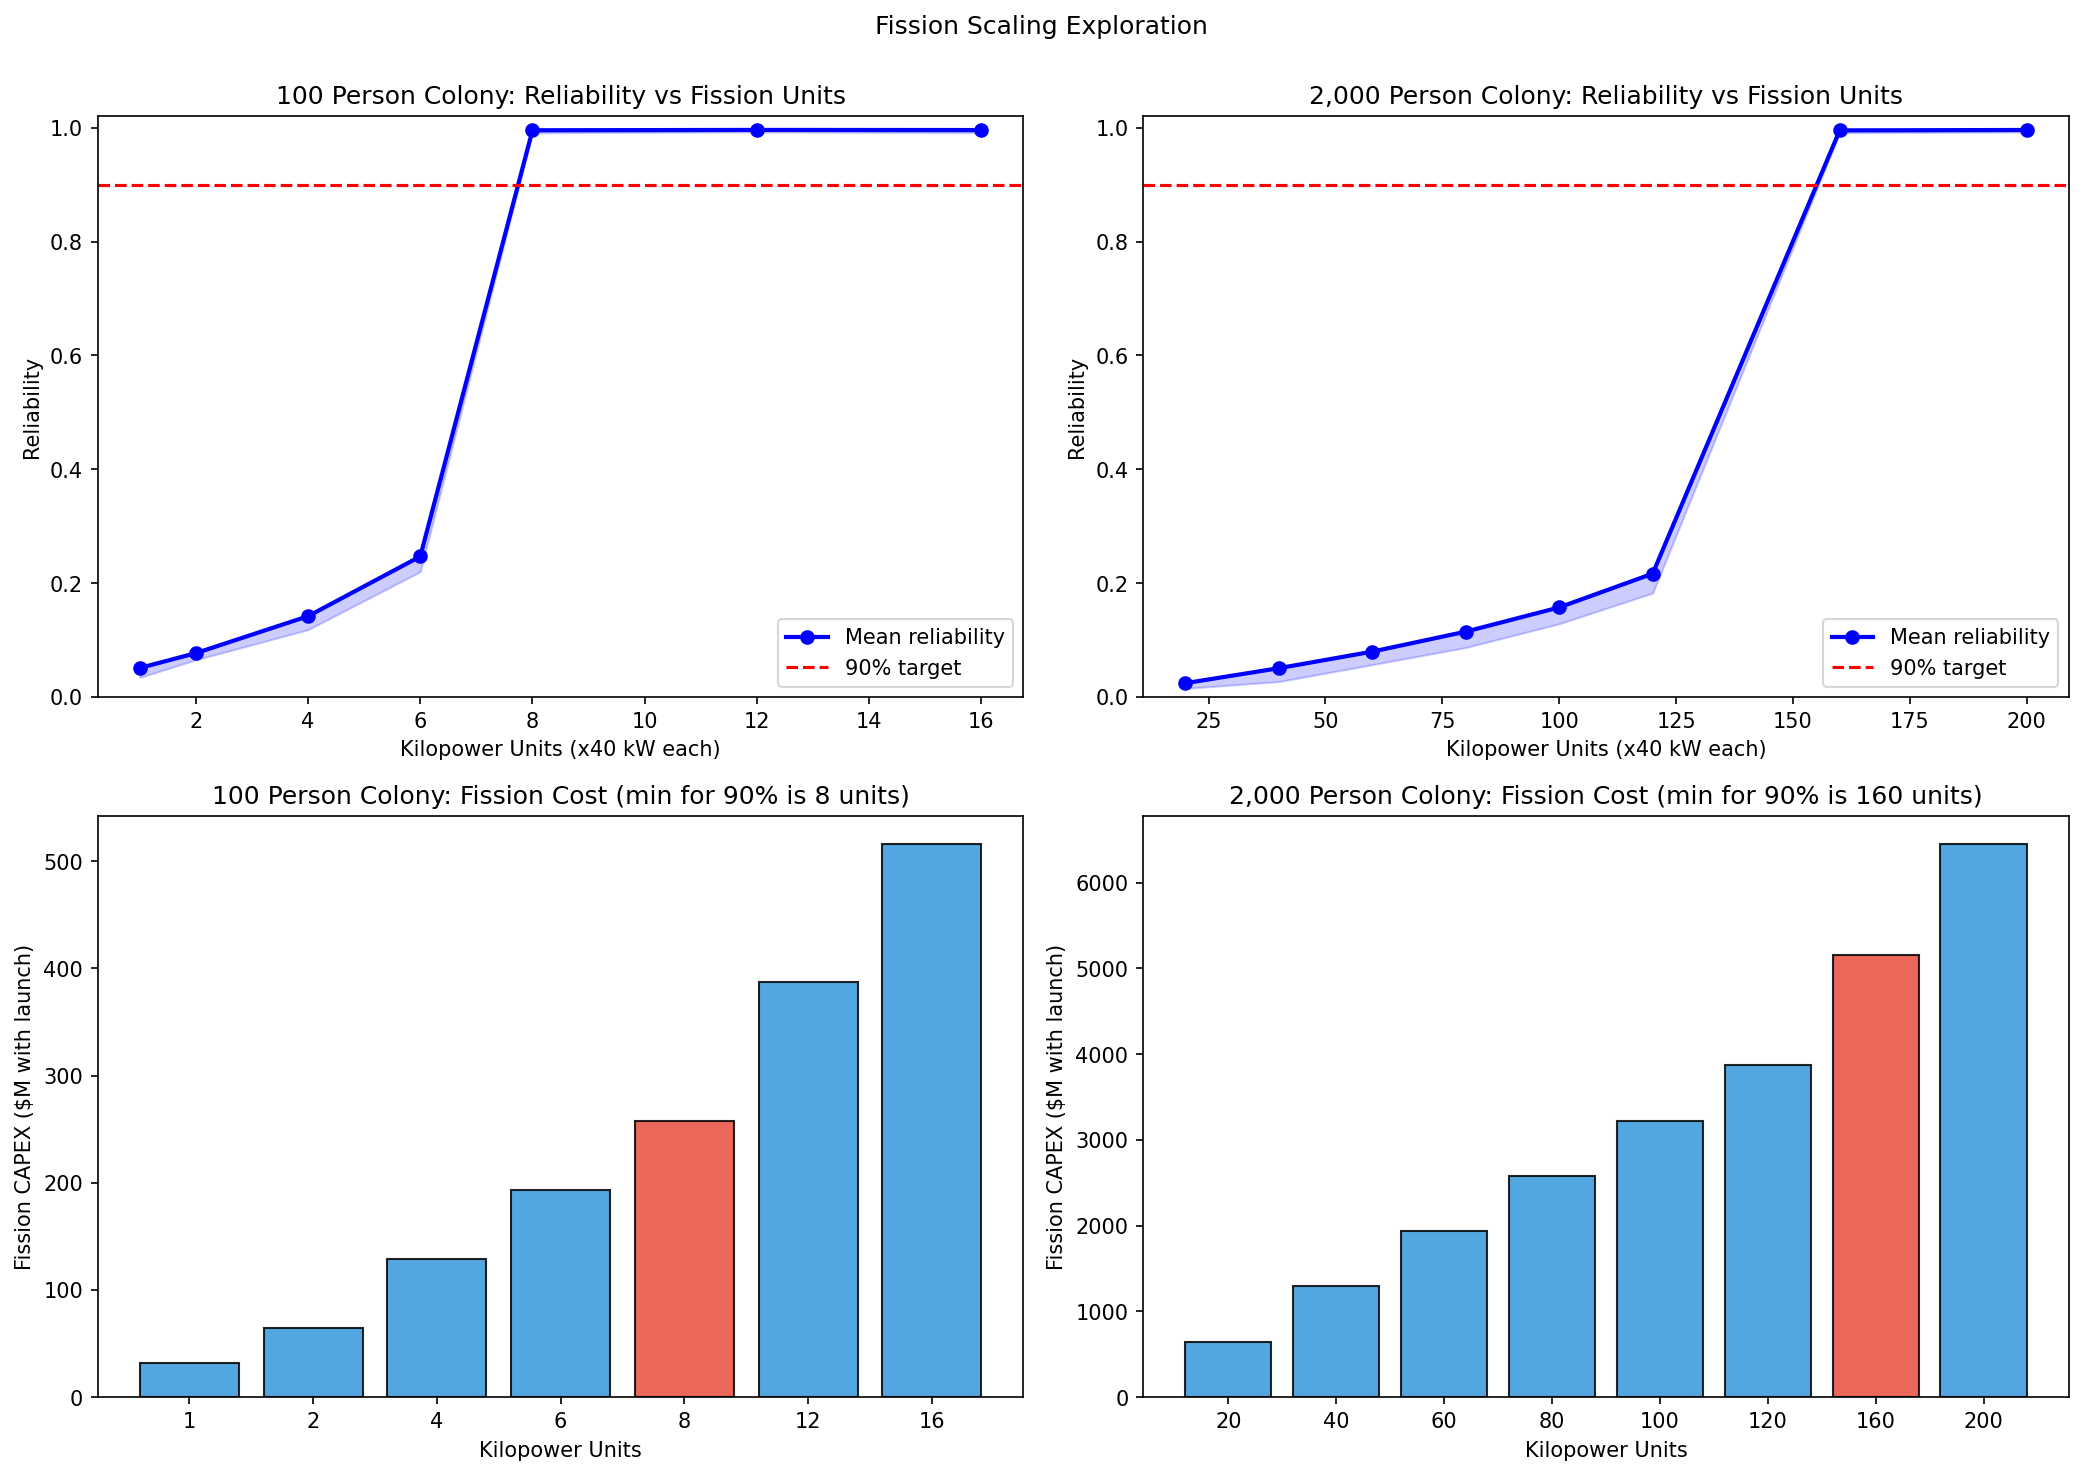
\includegraphics[height=0.56\textheight]{fission_scaling.png}

\vspace{0.15cm}
\small
\begin{itemize}
\item For the 100 person colony, about 8 Kilopower units get past 90 percent mean reliability.
\item For the 2{,}000 person colony, the same threshold takes about 160 units, which is where scaling pressure starts to matter.
\end{itemize}
\end{frame}

\begin{frame}
\frametitle{sensitivity checks}
\begin{columns}[T]
\begin{column}{0.49\textwidth}
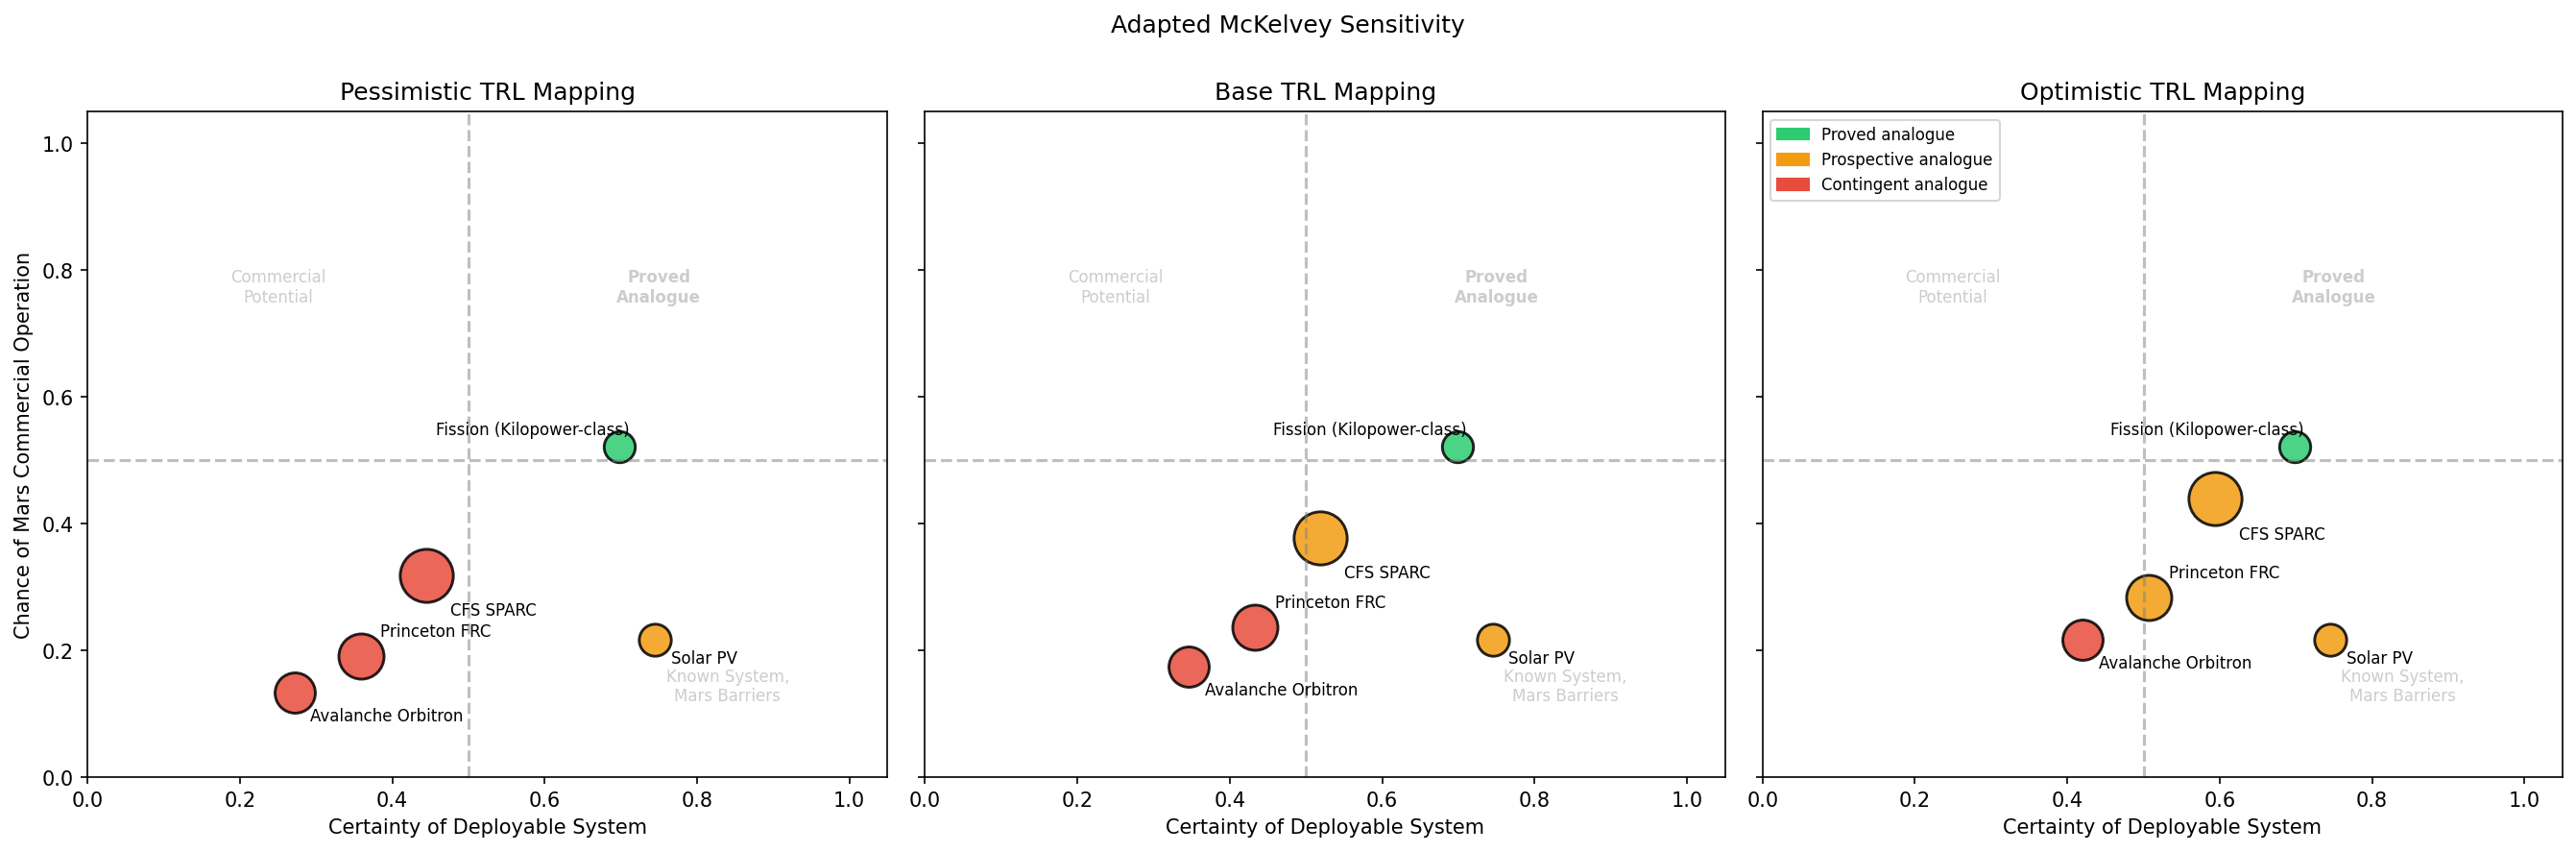
\includegraphics[width=\textwidth]{mckelvey_sensitivity.png}
\end{column}
\begin{column}{0.49\textwidth}
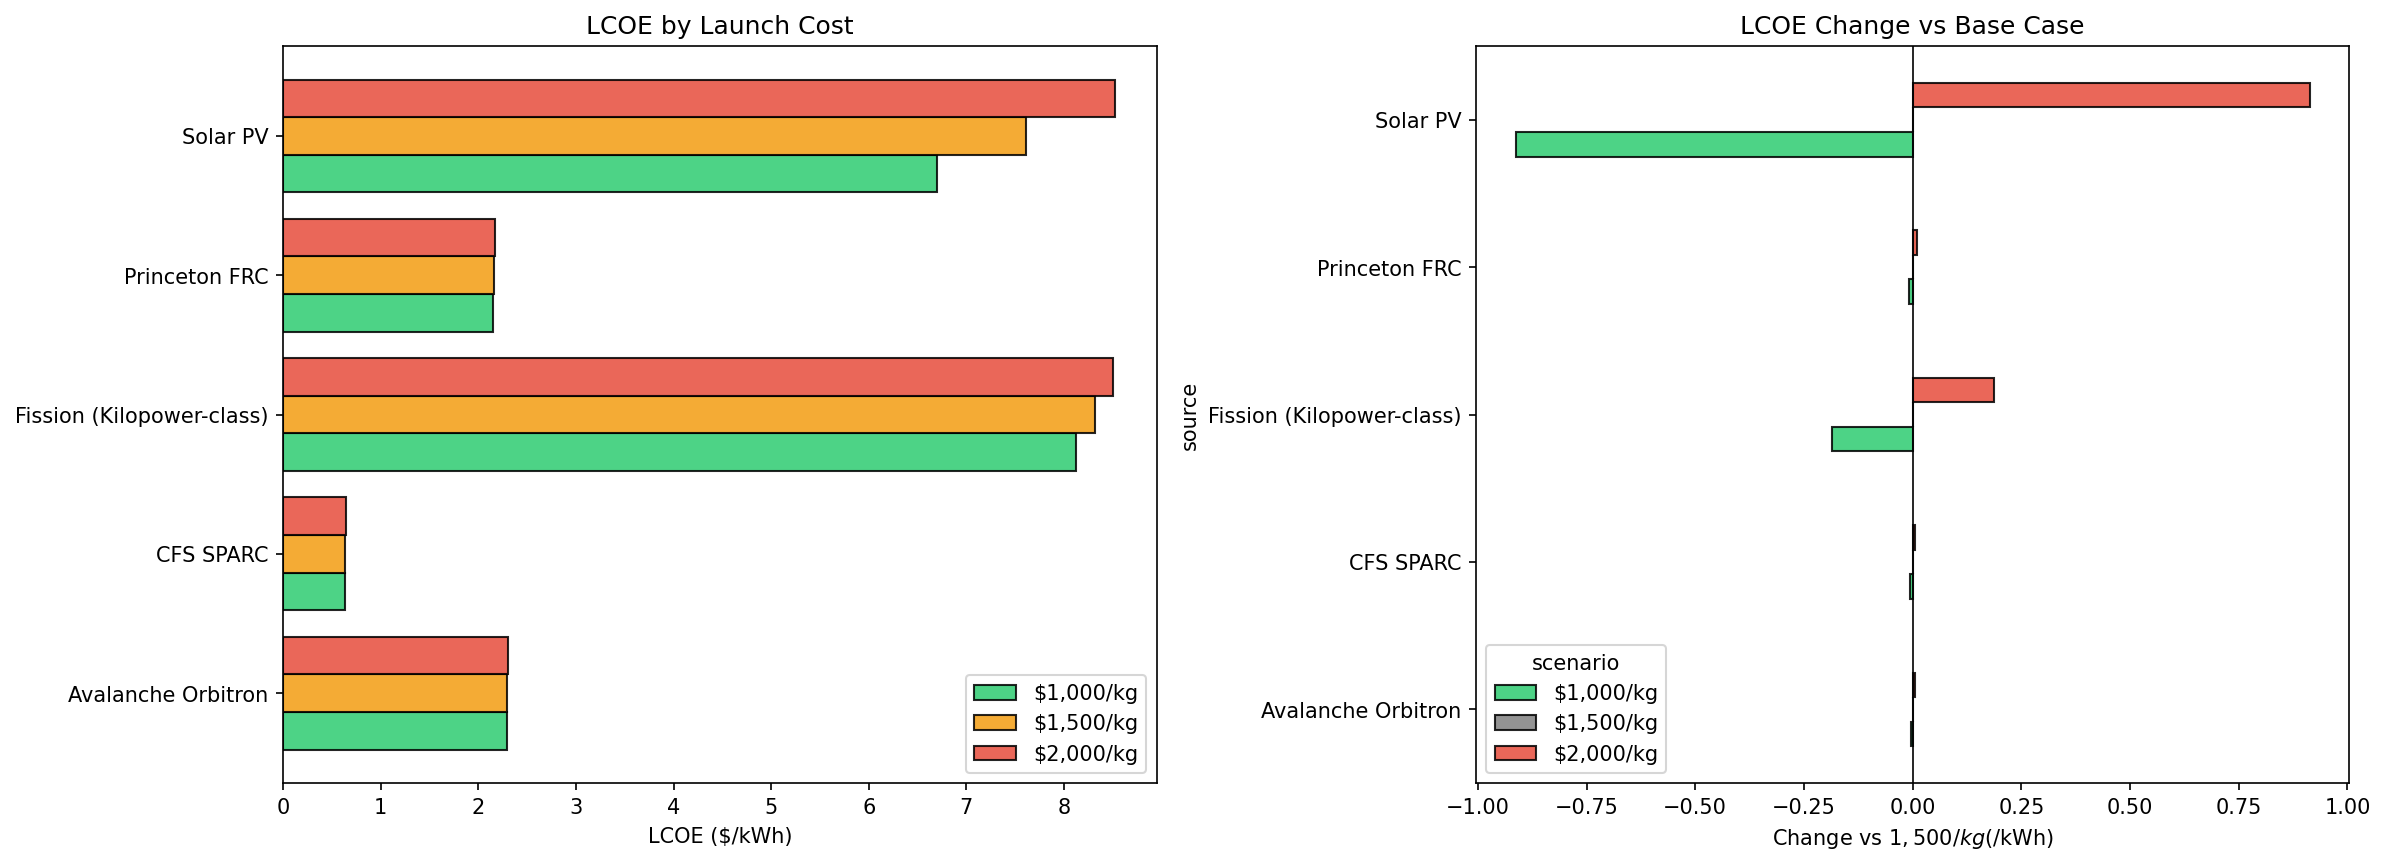
\includegraphics[width=\textwidth]{lcoe_sensitivity.png}
\end{column}
\end{columns}

\vspace{0.15cm}
\begin{itemize}
\item The sensitivity runs shift the exact placement of some options, but they do not change the big story.
\item Fusion is still promising but immature, and solar only systems are still not reliable enough.
\end{itemize}
\end{frame}

\begin{frame}
\frametitle{forecast summary}
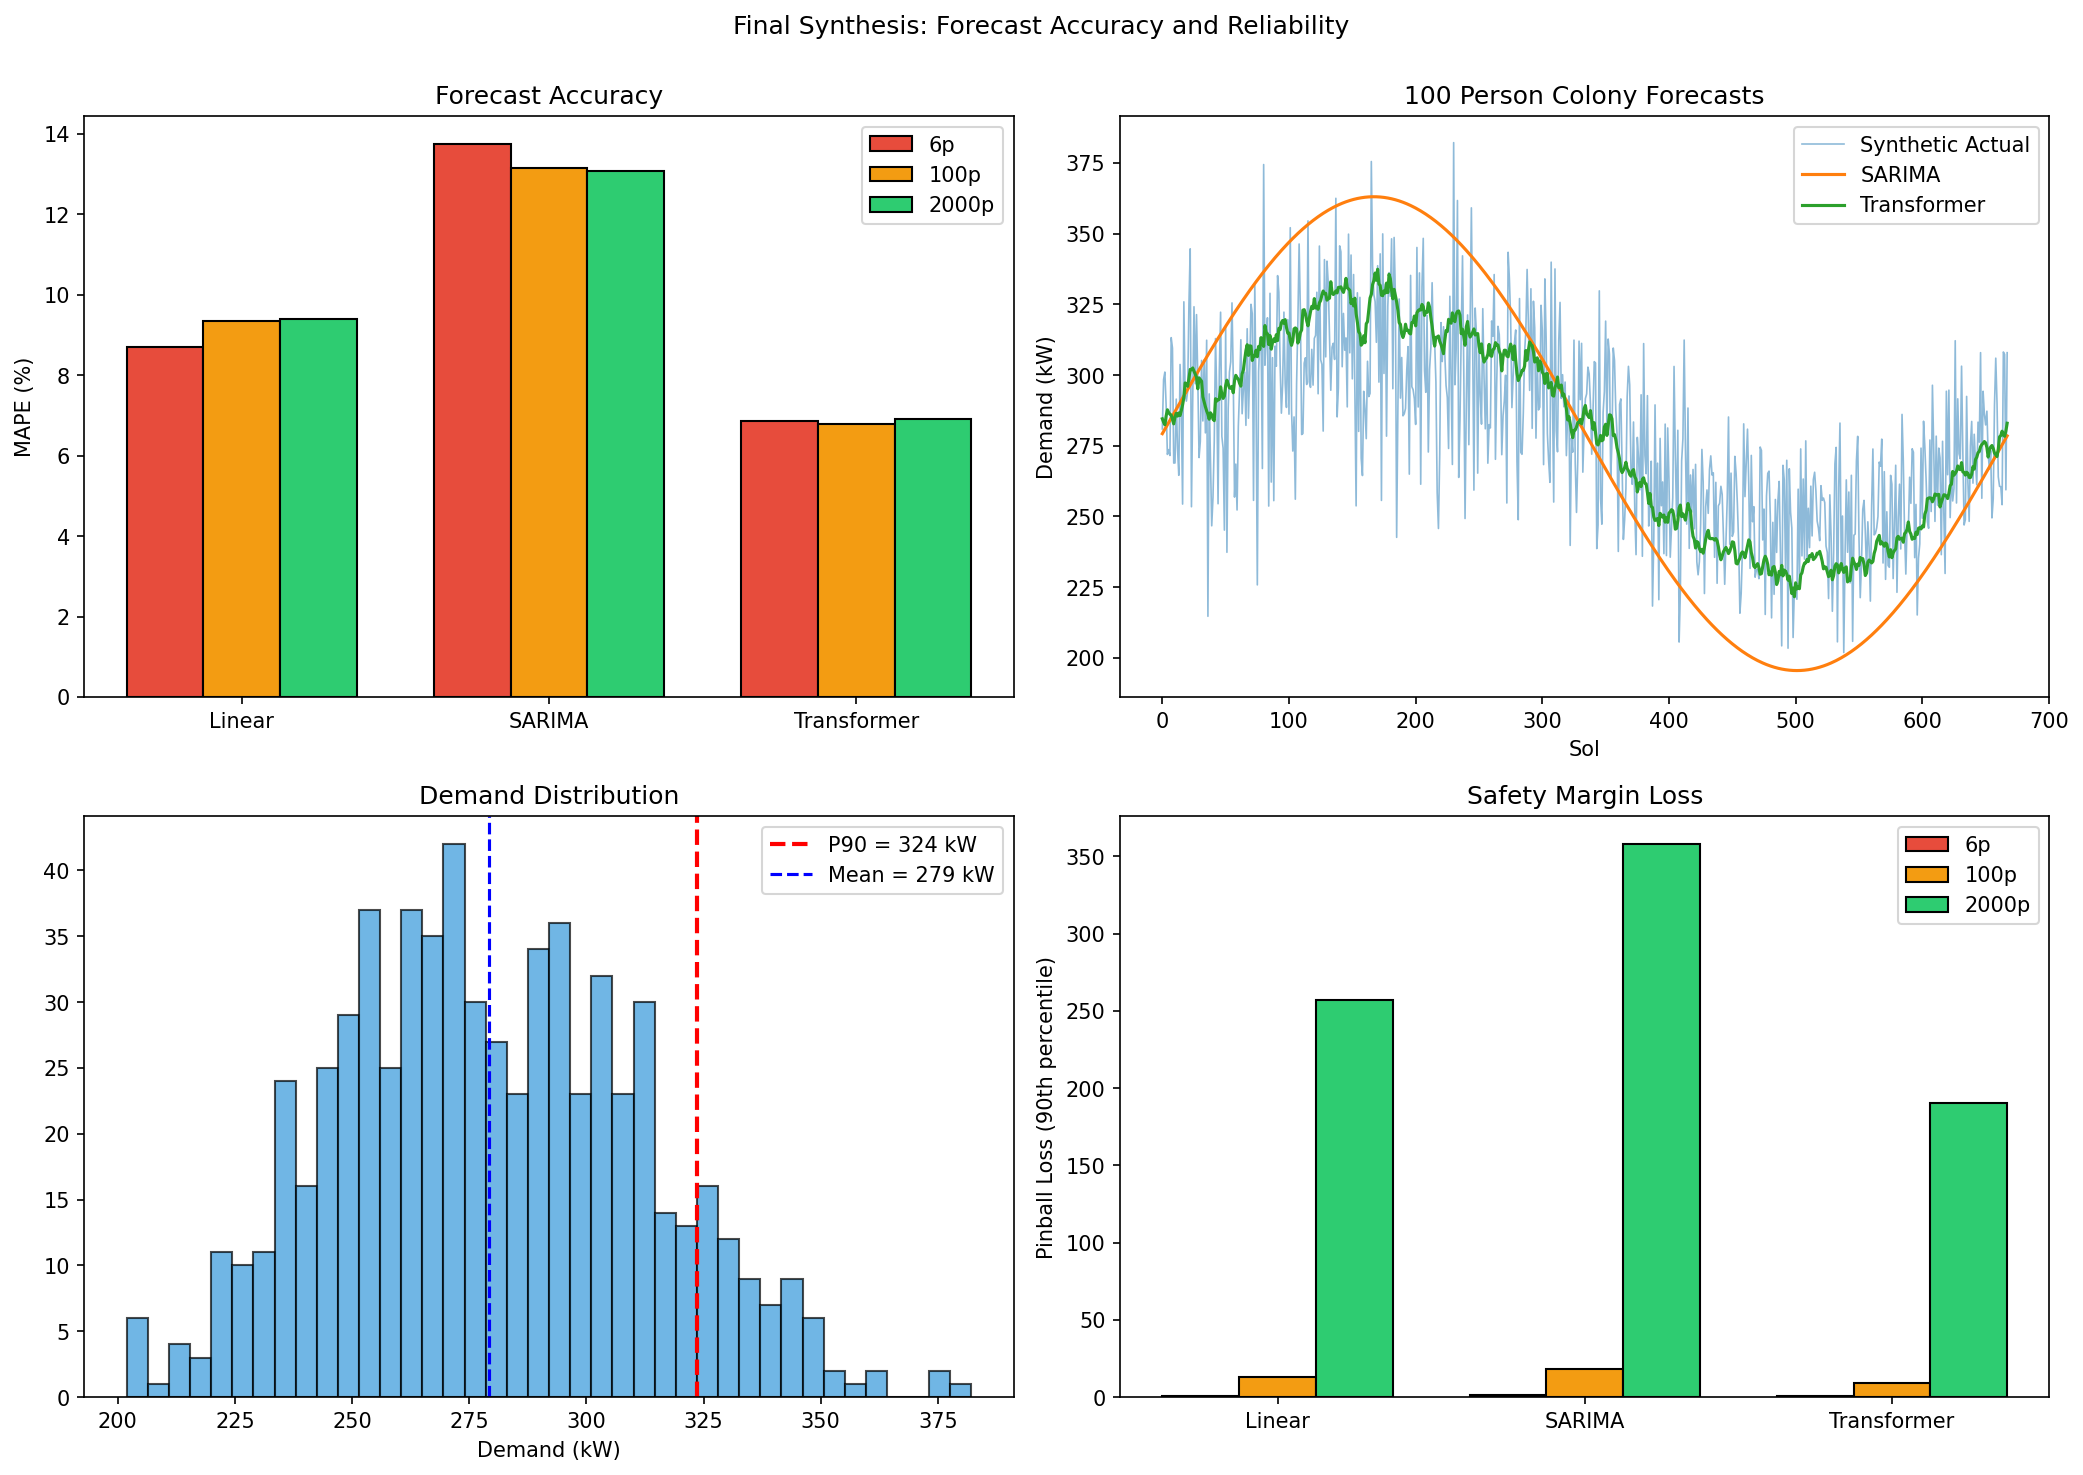
\includegraphics[height=0.56\textheight]{final_synthesis.png}

\vspace{0.15cm}
\small
\begin{itemize}
\item The Transformer proxy gives the lowest error in this side analysis for all colony sizes.
\item We treat this as supporting context, not the main claim of the project.
\end{itemize}
\end{frame}

\begin{frame}
\frametitle{answers to the three questions}
\begin{enumerate}
\item Fusion starts to look better when the colony gets large enough that scaling many small fission units becomes logistically ugly.
\item Dust storms matter a lot for solar, and they are the main reason solar only systems fail in our runs.
\item SPARC looks strongest on projected cost, but fission is still the most credible near term answer.
\end{enumerate}
\end{frame}

\begin{frame}
\frametitle{limits and future work}
\begin{itemize}
\item Fusion performance numbers come from public concept material, not from operating Mars ready reactors.
\item The dust penalty curve and habitat constants are simplified engineering inputs, not direct measurements of a future colony.
\item A stronger next step would be a better operational model for fusion and a more physical solar degradation model.
\end{itemize}
\end{frame}

\begin{frame}
\frametitle{main takeaways}
\begin{itemize}
\item Solar only is not good enough for a serious colony in the cases we tested.
\item Fission is the practical answer now because it carries the reliability burden.
\item Fusion stays interesting as a long run scale argument, especially for very large colonies.
\item Full code, report, and figures: \url{https://github.com/sjheinz17/MarsColonyNuclearFusion}
\end{itemize}
\end{frame}

\end{document}
